%\begin{filecontents}{apsrevcontrol.bib}
%  @CONTROL{apsrev41Control,title="0"%,author="48",editor="1",pages="1",year="0"}
%\end{filecontents}
\RequirePackage[l2tabu, orthodox]{nag}
\RequirePackage{fixltx2e}
\PassOptionsToPackage{pdftex,psdextra=true,
pdfversion=1.7,
pdfencoding=auto,
pdfnewwindow=true,
pdfusetitle=true,
psdextra=true,
pdftoolbar=false,
pdfmenubar=false,
bookmarks=true,
bookmarksnumbered=true,
bookmarksopen=true,
pdfpagemode=UseThumbs,
bookmarksopenlevel=1,
pdfpagelabels=false
}{hyperref}
\documentclass[aps,english,superscriptaddress,onecolumn,twoside,longbibliography,pra,floatfix,fleqn,nofootinbib]{revtex4-1}%


\usepackage[utf8]{inputenx}% for arXiv use encoding ansinew
%\input{ix-utf8enc.dfu}
\usepackage[OT1]{fontenc}

\usepackage{amsfonts}
\usepackage{amssymb}
\usepackage{amsthm}
\usepackage[intlimits]{amsmath}
\usepackage{graphicx}%
\usepackage{placeins} %for FloatBarrier
\usepackage{afterpage} %for FloatBarrier in afterpage wrapper
%\usepackage{flushend}
%\usepackage{dblfloatfix}
\usepackage[normalem]{ulem} %for sout
\usepackage[raggedright,bf,nooneline]{subfigure}
\renewcommand{\thesubfigure}{\alph{subfigure}}
\usepackage{paralist}
%\usepackage{ellipsis}
%\usepackage{float}

\setcounter{MaxMatrixCols}{30}
\providecommand{\U}[1]{\protect\rule{.1in}{.1in}}
%EndMSIPreambleData
\newtheorem{theorem}{Theorem}
\newtheorem{acknowledgement}[theorem]{Acknowledgement}
\newtheorem{algorithm}[theorem]{Algorithm}
\newtheorem{axiom}[theorem]{Axiom}
\newtheorem{claim}[theorem]{Claim}
\newtheorem{conclusion}[theorem]{Conclusion}
\newtheorem{condition}[theorem]{Condition}
\newtheorem{conjecture}[theorem]{Conjecture}
\newtheorem{corollary}[theorem]{Corollary}
\newtheorem{criterion}[theorem]{Criterion}
\newtheorem{definition}[theorem]{Definition}
\newtheorem{example}[theorem]{Example}
\newtheorem{exercise}[theorem]{Exercise}
\newtheorem{lemma}[theorem]{Lemma}
\newtheorem{notation}[theorem]{Notation}
\newtheorem{problem}[theorem]{Problem}
\newtheorem{prop}{Proposition}
\newtheorem{taut}{Tautology}
\newtheorem{remark}[theorem]{Remark}
\newtheorem{solution}[theorem]{Solution}
\newtheorem{summary}[theorem]{Summary}
%\newenvironment{proof}[1][Proof]{\noindent\textbf{#1.} }{\ \rule{0.5em}{0.5em}}

% hyperlink stuff
\usepackage[usenames,dvipsnames]{xcolor}
\definecolor{ultramarine}{RGB}{63, 0, 255}
\definecolor{medblue}{RGB}{0, 0, 100}
\definecolor{panblue}{RGB}{0,24,150}
\definecolor{carmine}{RGB}{150, 0, 24}
\usepackage[breaklinks=true]{hyperref}
\hypersetup{colorlinks,
linkcolor=carmine,
citecolor=medblue,
urlcolor=panblue,
anchorcolor=OliveGreen}
%\usepackage{url}


\definecolor{purple}{RGB}{128,0,128}
\definecolor{PURPLE}{RGB}{128,0,128}
\definecolor{BLACK}{RGB}{0,0,0}
\definecolor{ultramarine}{RGB}{63, 0, 255}
\definecolor{medblue}{RGB}{0, 0, 100}
\definecolor{panblue}{RGB}{0,24,150}
\definecolor{carmine}{RGB}{150, 0, 24}
\definecolor{gray}{RGB}{150, 150, 150}

\newcommand{\purp}[1]{{\color{purple}{#1}\color{black}}}
\newcommand*{\mred}[1]{{\color{RawSienna}{\mathbf{#1}}}}
\newcommand*{\mblue}[1]{{\color{MidnightBlue}{\mathbf{#1}}}}
\newcommand*{\mpurp}[1]{{\color{Plum}{\mathbf{#1}}}}
\newcommand*{\mgreen}[1]{{\color{OliveGreen}{\mathbf{#1}}}}
\newcommand*{\tred}[1]{{\color{carmine}{\textbf{#1}}}}
\newcommand*{\tblue}[1]{{\color{MidnightBlue}{\textbf{#1}}}}
\newcommand*{\tpurp}[1]{{\color{Plum}{\textbf{#1}}}}
\newcommand*{\tgreen}[1]{{\color{OliveGreen}{\textbf{#1}}}}

\newcommand{\quoteby}{\raise.17ex\hbox{$\scriptstyle\sim$}}

\usepackage{verbatim} %for comment command
\usepackage{units}% for nicefrac
\newcommand{\half}[1]{\nicefrac{#1}{2}}

%\usepackage{braket} %provide \bra and \Bra and \set and \Set etc...
%\newcommand{\brackets}[1]{\lbrace{#1\rbrace}}
%\newcommand{\brackets}{\Set}



\usepackage{microtype}
%\usepackage{MnSymbol}

\usepackage[capitalise]{cleveref}
\Crefname{eqs}{Eqs.}{Eqs.}
\creflabelformat{eqs}{(#2#1#3)}
\crefrangelabelformat{equation}{(#3#1#4-#5#2#6)}
%\crefmultiformat{equation}{eqs.~(#2#1#3)}{ and~(#2#1#3)}{, (#2#1#3)}{ and~(#2#1#3)}
\Crefmultiformat{equation}{Eqs.~(#2#1#3}{,#2#1#3)}{,#2#1#3}{,#2#1#3)}
\Crefname{prop}{\textbf{Prop}.}{\textbf{Props}.}
\Crefname{taut}{\textbf{Taut}.}{\textbf{Tauts}.}
\Crefname{section}{Sec.}{Secs.}

\usepackage{mathtools} %for mathclap and prescript and more. Learning to love this package. And DeclarePairDelimeter!
\DeclarePairedDelimiter{\ceil}{\lceil}{\rceil}
\DeclarePairedDelimiter{\floor}{\lfloor}{\rfloor}
\DeclarePairedDelimiter{\parens}{\lparen}{\rparen}
\DeclarePairedDelimiter{\parenths}{\lparen}{\rparen}
\DeclarePairedDelimiter{\abs}{\lvert}{\rvert}
\DeclarePairedDelimiter{\norm}{\lVert}{\rVert}
\DeclarePairedDelimiter{\braces}{\lbrace}{\rbrace}
\DeclarePairedDelimiter{\bracks}{\lbrack}{\rbrack}
\newcommand{\brackets}[1]{\braces*{#1}}

%\usepackage{nath} %automatically pair delimiters. Provides \inline and \displayed. Adjusts \frac and /

\newcommand{\na}{\ensuremath{\mathring{a}}}
\newcommand{\nb}{\ensuremath{\mathring{b}}}
\newcommand{\nc}{\ensuremath{\mathring{c}}}

\newcommand{\naf}{\ensuremath{\lnot a}}
\newcommand{\nbf}{\ensuremath{\lnot b}}
\newcommand{\ncf}{\ensuremath{\lnot c}}

\newcommand{\n}[1]{\ensuremath{\overline{#1}}}
\newcommand{\ot}[1]{\ensuremath{\overline{#1}}}
\newcommand{\Nor}[1]{\operatorname{\mathsf{Nor}}\!\bracks*{#1}}

\newcommand{\larray}[1]{\ensuremath{\begin{array}{l}#1\end{array}}}
\newcommand{\lparens}[1]{\ensuremath{\parens*{\larray{#1}}}}
\newcommand{\NamedFunction}[2]{\operatorname{\mathsf{#1}}\!\bracks*{\larray{#2}}}

\newcommand{\nap}{\ensuremath{a'}}
\newcommand{\nbp}{\ensuremath{b'}}
\newcommand{\ncp}{\ensuremath{c'}}
\newcommand{\napp}{\ensuremath{a''}}
\newcommand{\nbpp}{\ensuremath{b''}}
\newcommand{\ncpp}{\ensuremath{c''}}

\newcommand{\p}[1]{p\parenths{#1}}
\newcommand{\cramp}[1]{\ensuremath{\mathord{#1}}}
%\newcommand{\cramp}[1]{\ensuremath{\mathopen{}#1\mathclose{}}} oldway. New way is better.
\newcommand{\eql}{\cramp{=}}

\usepackage{bm}
\newcommand{\setlambda}{\bm{\lambda}}



\let\stdsection\section
\renewcommand\section{\clearpage\stdsection}%every section new page


\begin{document}
%\preprint{ }
%\title{Transitivity of implication and causal structure}
\title{A Method to Derive Polynomial Inequalities for Causal Structures}
\author{Tobias Fritz}
\email{tfritz@perimeterinstitute.ca}
\affiliation{Perimeter Institute for Theoretical Physics, Waterloo, Ontario, Canada, N2L 2Y5}
\affiliation{Max Planck Institute for Mathematics in the Sciences, Leipzig, Saxony, Germany, 04103}
\author{Robert W. Spekkens}
\email{rspekkens@perimeterinstitute.ca}
\affiliation{Perimeter Institute for Theoretical Physics, Waterloo, Ontario, Canada, N2L 2Y5}
\author{Elie Wolfe}
\email{ewolfe@perimeterinstitute.ca}
\affiliation{Perimeter Institute for Theoretical Physics, Waterloo, Ontario, Canada, N2L 2Y5}
\date{\today}


\begin{abstract}
The fundamental task of causal inference is to ascertain which observable probability distributions are compatible with a given causal structure, especially when the structure includes latent variables which cannot be directly observed. While causal compatibility criteria are important in many fields, our interest is motivated by their use in quantum theory, where they distinguish non-classical from classical correlation. Bell inequalities are a type of causal compatibility criteria which apply only to very special causal structures. For more general causal structure one must use different types of causal compatibility criteria, such as testing for conditional independence between observed variables, or by checking the mutual information between variables against entropic upper bounds implies by the causal structure. These more general techniques, however, are often incapable of recognizing uniquely quantum correlations. We here introduce a method for deriving polynomial inequalities constraining compatibility with general causal structures. While this method was originally motivated by desiderata from quantum theory it should nevertheless be valuable in causal inference tasks more broadly.


\end{abstract}
\maketitle
%In Ref.~\cite{WoodSpekkens}, the standard proof of Bell's theorem is presented in the language of causal inference.  In particular, the CHSH inequality emerges as a special case of what Pearl calls an ``instrumental inequality''.  Hardy's proof of Bell's theorem is quite different from the standard proof and the following question naturally arises: is there a generic tool for classical causal inference of which the Hardy argument can be considered a special case when applied to the M-shaped causal structure of the Bell experiment?

%To try and answer this question, we apply Hardy-type reasoning to the triangle causal structure, that is, the one with three observed variables, each pair of which have a common cause.  We show that this sort of reasoning does indeed facilitate causal inference in the case of the triangle causal structure, thereby lending some evidence to the notion that this style of argument has the potential to be generalized into a generic tool for classical causal inference.

\section{Introduction \& Notation}
Given some hypothesis of causal structure it is desirable to determine the set of observable probability distributions compatible with the hypothesis. Causal structure compatibility criteria are leveraged in a wide variety of statistics application, from sussing out biological pathways to enabling artificially intelligent machine learning \cite{pearl2009causality,spirtes2011causation,studeny2005probabilistic,koller2009probabilistic}. The foundational role of causal structure in quantum information theory has only recently been appreciated \cite{WoodSpekkens,fritz2012bell,pusey2014gdag,BeyondBellII}: classical correlations on a causal structure are those probability distributions compatible with restricting the latent variables to be hidden ontic states; quantum correlations are those which are uniquely realizable if the latent variables in the causal structure are allowed to be quantum states.

Tightly characterizing the set of observable probability distributions compatible with a causal structure is therefore physically critical, in order to recognize and exploit uniquely quantum distributions. Practical techniques for generically constraining causal compatibility include the use of conditional independence relations (easy) \cite{pearl2009causality,spirtes2011causation,studeny2005probabilistic,koller2009probabilistic} and entropic inequalities (more advanced) \cite{fritz2013marginal,chaves2014novel,chaves2014informationinference}. These criteria, however, do not provide a tight characterization, and frequently fail to ascertain the non-classicality of quantum correlation. 

Distinguishing quantum from classical correlations has historically been achieved through to use of Bell inequalities \cite{bell1966lhvm,GisinFramework2012,scarani2012device,Brunner2013Bell}. Bell inequalities however, and their convex hull derivation technique, are limited to causal scenarios involving only one latent common cause variable. New techniques are required to derive quantum-useful causal compatibility criteria for more general causal scenarios \cite{fritz2012bell,pusey2014gdag,BeyondBellII}.

To this end, we introduce a technique applicable to general causal structures for deriving polynomial inequalities constraining observable probability distributions. \purp{Trying out some new terminology, looking for more intuitive naming... }  Our technique works by first mapping the target causal structure $G$ to a purely common cause representation $G'$, which we call \tred{latent reduction}, $G'=\NamedFunction{LR}{\!G\!}$. 
%a process we'll explain in \cref{sec:LR}. 
To gently introduce the reader to the other steps in our technique, we choose to delay the discussion of latent reduction until \cref{sec:LR}. We use the Triangle scenario in \cref{sec:TriSimple} as our first example to illustrate deriving polynomial inequalities \emph{specifically because the latent reduction step is not needed there}: the Triangle causal structure is isomorphic to its own latent reduction.  




\purp{Changelog Nov 5:

\begin{compactitem}[$\bullet$]
\item  Added three new causal structure figure: S15, S20, and S7. S15 is conjectured to be correlation equivalent. S20 and S7 are provably not. S20 and S7 admit causal structure variants without changing the effective correlation scenario.
\item Rewrote abstract and the introduction.
\item Switched a bunch of terminology.
\end{compactitem}
}


We follow the convention that upper-case letters indicate random variables while lower-case letters indicate some particular value associated with the corresponding random variable. In this convention, for example, a student's score on some exam $X$ might depend probabilistically on the extent of sleep $S$. The Boolean proposition, or {event}, $X\cramp{=}x|S\cramp{=}s$ should be understood as "the students scores $x$ on the exam given a duration of sleep equal to $s$. As conditional propositions form the basis of much of what follows, we \tred{represent conditioning via subscript notation}, such as $x_s$ to indicate the event $X\cramp{=}x | S\cramp{=}s$. 

%In the study of causal structures one often encounters hidden, or latent, variables, which are posited to explain apparent correlations and randomness. 
Throughout this article {latent random variables are represented by $\Lambda\cramp{=}\lambda$, or by the first letters of the Roman alphabet}, such as $A\cramp{=}a,B\cramp{=}b,$ etc. 
Observable (non-latent) variables will generally be represented by the letters from the end of alphabet, such as $S\cramp{=}s,T\cramp{=}t,...,Z\cramp{=}z$. In graphical depictions it is conventional to represent latent variables by circles and observable variables by triangles \cite{pusey2014gdag}.

%An exception is made when an observable variable corresponds to a \emph{setting}, for which we reserve the middle letters, such as $S,T$ etc.

%Furthermore, \tred{latent variables will be further indicated  via a condition symbol ($|$) inside subscripts}. A vertical separator inside a subscript merely indicates latent variables on the right side. Thus, $x_{s|a}$ is the event $\parens*{X\cramp{=}x|S\cramp{=}s,A\cramp{=}a}$.  

%Essential to our work here is that we can take the dependence on the latent variable to be deterministic. In other words, the \tred{latent-complete} proposition $x_{s|a}$ is always true or always false; as an event it occurs with probability either zero or one. Propositions can be true, false, or inconclusive; analogously events can occurs with 100\% probability, 0\% probability, or something in between.

%The assumptions of deterministic dependence ensures that any \tred{latent-complete} joint probability term can be factored in an arbitrary fashion: $\p{x_{s|a} , y_{t|a}}=\p{x_{s|a}}\p{y_{t|a}}$. This freedom-to-factorize is justified because binary multiplication is equivalent to logical conjunction. This cannot be over-emphasized: \tred{Any latent-complete joint probability factorizes arbitrarily.} Indeed, the connection between formal logic statements and probabilities forms the essence of our technique for deriving inequalities.


We adopt the convention of indicating logical negation by $\NamedFunction{Not}{\!x\!}\equiv\n{x}$ such that $\n{x}$ references the possibility of \emph{any} outcome other than $x$, i.e. $\p{\n{x}}\equiv\p{X\cramp{\neq}x}=1-\p{X\cramp{=}x}$. The negation of a conditional event should be interpreted as any other outcomes given the same settings, such that $\p{\n{x_{s a}}}=\p{X\cramp{\neq}x|S\cramp{=}s,A\cramp{=}a}$.

Note that \tred{logical conjunction is herein represented by default}, such that $\p{x y}$ is the probability of $X\cramp{=}x$ \emph{and} $Y\cramp{=}y$. Logical conjunction is also implicit among all variables appearing in subscript.

Finally, note that \tred{superscript notation indicates a dummy index}, such that $x^2_{s^2 a^1}$ is shorthand for $\parens*{X\cramp{=}x^{(2)}|S\cramp{=}s^{(2)},A\cramp{=}a^{(1)}}$. 



\section{Triangle Scenario - simple example}\label{sec:TriSimple}


%It is often claimed that classically one must have $\p{a_1 b_1}\geq \p{a_0 b_0}$ from just the first two conditions in  \cref{eq:hardycontrapositive} alone \cite{CabelloHardyInequality}, such that the result ``If additionally $\p{a_1 b_1}=0$ then $\p{a_0 b_0}=0$" is just a special case. 
%We now demonstrate that this Hardy-type inequality follows naturally from assumptions about causal structure. More importantly, we show that Hardy-type arguments can be used to derive compatibility criteria in the same vein even for general causal structures.


\begin{figure*}[t!]
\centering
\subfigure[\hspace{-0.5ex}:\hspace{1ex} The causal structure of the Triangle scenario. Note that there are no direct influences between observable variables.\hfill]
{\begin{minipage}[t]{.45\textwidth}
    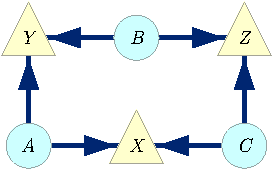
\includegraphics[width=1.8in]{GenuineTriangleDAG.pdf}
    \label{fig:TriDAG}
\end{minipage}}\hfill{\color{gray}\rule[-0.4cm]{0.5pt}{3cm}}\hfill
\subfigure[\hspace{-0.5ex}:\hspace{1ex} An isomorphic directed acyclic graph encoding the causal structure of the Triangle scenario.\hfill]
{\begin{minipage}[t]{.45\textwidth}
    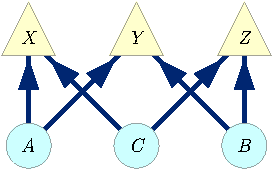
\includegraphics[width=1.8in]{EffectiveTriangleDAG.pdf}
    \label{fig:EffTriDAG}
\end{minipage}}
\vspace{-2ex}\caption{The Triangle scenario: A scenario in which three observable variables are pairwise-correlated but lack a triplewise common ancestor. Conventionally latent variables are indicated by circles while observable variables are indicated by triangles~\cite{pusey2014gdag}.}
\label{fig:Triangle}\vspace{-2ex}
\end{figure*}

%\begin{figure}[b,t]
%\center{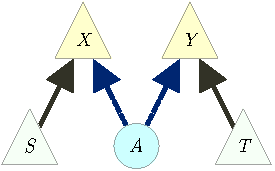
\includegraphics[width=0.7\linewidth]{BellScenarioDAG.pdf}}
%\caption{(color online) The causal structure of the Bell scenario, on which Bell's theorem is based. Per convention, latent variables are indicated by circles whereas observable variables are indicated by triangles \cite{pusey2014gdag}. Observable variables with no incoming edges are setting variables, and are indicated by a light green shading.}
%\label{fig:BellDAG}
%\end{figure}
We first illustrate our method for deriving polynomial inequalities by considering the Triangle scenario [\citealp{pusey2014gdag}~(Fig.~E\#8), \citealp{WoodSpekkens}~(Fig.~18b), \citealp{fritz2012bell}~(Fig.~3), \citealp{chaves2014novel}~(Fig.~6a), \citealp{Chaves2015infoquantum}~(Fig.~1a), \citealp{BilocalCorrelations}~(Fig.~8), \citealp{steudel2010ancestors}~(Fig.~1b), \citealp{chaves2014informationinference}~(Fig.~4b)], the causal structure of which is depicted here in \cref{fig:Triangle}. Here $\brackets{X,Y,Z}$ are the observable variables, and  $\brackets{A,B,C}$ are latent. $A$ denotes the common cause of $X$ and $Y$, etc. The Triangle scenario is a correlation scenario in the sense of \citet{fritz2012bell}; see especially Sec. 2.3 there.

There can be no linear inequality in term of probabilities for the triangle scenario, which makes a polynomial inequality technique especially valuable for this scenario. The nonlinear of the Triangle scenario follows for the non-convexity of the set of all probability distributions which are compatible with it. \purp{Proof of nonconvexity or nonlinearity needed. Tobias?}

Causal structure generally dictates that not all the observable variables depend on all the latent variables, but rather each observable variable depends only in its particular latent ancestors. For the Triangle scenario this means that
\begin{align}\begin{split}\label{eq:tristructure}
%\p{x y z | a b c}=\p{x_{c a}  y_{a b}  z_{b c}}
\p{x_{a b c}}=\p{x_{c a}} \,,\; \p{y_{a b c}}=\p{y_{b c}} \,,\; \p{z_{a b c}}=\p{z_{a b}} \,,\quad\text{and hence}\quad \p{x y z | a b c}=\p{x_{c a}  y_{a b}  z_{b c}}\,,
\end{split}\end{align}
and accordingly, 
\begin{align}\label{eq:triintegration}
&\p{x y z}=\sum\limits_{a\in \norm{A}} \sum\limits_{b\in \norm{B}} \sum\limits_{c\in \norm{C}} \p{x_{c a}  y_{a b}  z_{b c}}\p{a}\p{b}\p{c}.
\end{align}

Here is an example of a quadratic polynomial constraint for the Triangle scenario.
\begin{prop} \label{prop:Deg2}
The Triangle causal structure (\cref{fig:Triangle}) implies that
\begin{align*}
\p{x^1 y^1 z^1} \p{x^2 y^2 z^2}\leq \p{x^1} \p{x^2 y^3}+\p{y^1}\p{x^3 y^2} +\p{z^2}\p{\n{x^3} \n{y^3} z^1} 
\end{align*}
\end{prop}
\begin{proof}
We use the causal structure to consider various counterfactual propositions, which we collect into a logical tautology as follows.
\begin{align}\begin{split}\label{eq:tri2structaut}
&\NamedFunction{And}{ x^1_{c^1 a^1} , y^1_{a^1 b^1} , z^1_{b^1 c^1} , x^2_{c^2 a^2} , y^2_{a^2
   b^2} , z^2_{b^2 c^2} }
 \implies 
\NamedFunction{Or}{
    \NamedFunction{And}{ y^1_{a^1 b^1} , x^3_{c^1 a^2} , y^2_{a^2 b^2} } ,\\
    \NamedFunction{And}{ x^1_{c^1 a^1} , x^2_{c^2 a^2} , y^3_{a^2 b^1} } ,\\
    \NamedFunction{And}{ z^2_{b^2 c^2} , \n{x^3_{c^1 a^2}} , \n{y^3_{a^2 b^1}} , z^1_{b^1 c^1}
   }
}
\end{split}\end{align}
Next, we convert the tautology to an inequality via two rules:
\begin{enumerate}
\item As the antecedent always implies the consequent, the probability of the antecedent is necessarily less-than-or-equal-to the probability of the consequent. If $j \cramp{\scriptstyle \implies} k$ then $\p{j}\leq\p{k}$.
\item The probability of a disjunction of events is less-than-or-equal-to the sum of the probabilities of the individual events, i.e. ${\p{j\lor k}=\p{j}+\p{k}-\p{j,k}\leq \p{j}+\p{k}}$.
\end{enumerate}
The inequality which corresponds to \cref{eq:tri2structaut} is
\begin{align}\begin{split}\label{eq:tri2structineq}
\p{x^1_{c^1 a^1} y^1_{a^1 b^1} z^1_{b^1 c^1}} \p{x^2_{c^2 a^2} y^2_{a^2 b^2} z^2_{b^2 c^2}}\leq \lparens{
  \hphantom{+}\p{x^1_{c^1 a^1}} \p{x^2_{c^2 a^2} y^3_{a^2 b^1}}
\\+\p{y^1_{a^1 b^1}}\p{x^3_{c^1 a^2} y^2_{a^2 b^2}} 
\\+\p{z^2_{b^2 c^2}}\p{\n{x^3_{c^1 a^2}} \n{y^3_{a^2 b^1}} z^1_{b^1 c^1}} }
\end{split}\end{align}
Note that we have factored terms in \cref{eq:tri2structineq} according to distinct counter-factual instances. This is the key step in deriving polynomial inequalities. The distinct counterfactual instances are perhaps best seen by rewriting \cref{eq:tri2structineq} in a manner which does not assume a particular causal structure, namely
\begin{align}\begin{split}\label{eq:tri2operineq}
\p{x^1 y^1 z^1|c^1 a^1 b^1} \p{x^2 y^2 z^2|c^2 a^2 b^2}
\leq
\lparens{
  \hphantom{+}\p{x^1|c^1 a^1} \p{x^2 y^3|c^2 a^2 b^1}
\\+\p{y^1|a^1 b^1} \p{x^3 y^2|c^1 a^2 b^2} 
\\+\p{z^2|b^2 c^2} \p{\n{x^3} \n{y^3} z^1|c^1 a^2 b^1} }
\end{split}\end{align}
which we can marginalize both sides over all  $\brackets{a^1,b^1,c^1,a^2,b^2,c^2}$ to obtain \cref{prop:Deg2}.
\end{proof}
As both \cref{eq:tri2structaut,eq:tri2operineq} can be inferred from \cref{eq:tri2structineq}, we shall include only inequalities written in terms of individual-observable counterfactuals in subsequent proofs of polynomial inequalities.



Note that as a general matter, polynomial inequalities can be relaxed into interesting special cases by \emph{disregarding} some of the negated events. For example, we may suppose that a certain outcome is impossible, for example, we may imagine that $x^3\not\in \norm{X}$ in \cref{prop:Deg2}. We denote this as  $x^3\to \mathsf{False}$. By this substitution we have $\p{\n{x^3} \n{y^3} z^1} \to \p{\n{y^3} z^1}$ and $\p{x^3
   y^2}\to 0$, and thus we obtain the special case
\begin{align}\label{eq:tri2specialcase}
\p{x^1 y^1 z^1} \p{x^2 y^2 z^2}\leq \p{x^1} \p{x^2 y^3}+\p{z^2}\p{\n{y^3} z^1} 
\end{align}
which can be strengthened by ignoring events which do not appear on the right hand side of \cref{eq:tri2specialcase}, namely $\brackets{y^1,y^2}\to \mathsf{True}$.  Thus
\begin{align}
\p{x^1 z^1} \p{x^2 z^2}\leq \p{x^1} \p{x^2 y}+\p{z^2}\p{\n{y} z^1} .
\end{align}


\section{Triangle Scenario - degree 3 example}

Here is an example of a cubic polynomial constraint for the Triangle scenario. 
\begin{prop} \label{prop:AllPowerful}
The Triangle causal structure (\cref{fig:Triangle}) implies that
\begin{align*}\begin{split}
\p{x^1 y^1 z^1} \p{x^2 y^2 z^2} \p{x^3 y^3 z^3}
\leq
\lparens{
   \hphantom{+}\p{y^1} \p{x^4 y^3} \p{x^2 y^2 z^2}
\\+\p{z^3} \p{y^4 z^2} \p{x^1 y^1 z^1}
\\+\p{x^2} \p{z^4 x^1} \p{x^3 y^3 z^3}
\\+\p{z^1} \p{x^5 z^2} \p{x^3 y^3 z^3}
\\+\p{x^3} \p{y^5 x^1} \p{x^2 y^2 z^2}
\\+\p{y^2} \p{z^5 y^3} \p{x^1 y^1 z^1}
\\+\p{\n{x^4} \n{y^4} \n{z^4}} \p{\n{x^5} \n{y^5} \n{z^5}}}
\end{split}\end{align*}
\end{prop}
\begin{proof}\cref{prop:AllPowerful} is self-evident from the following inequality
\begin{align}\label{eq:tri3structineq}
\p{x^1_{c^1 a^1} y^1_{a^1 b^1} z^1_{b^1 c^1}} \p{x^2_{c^2 a^2} y^2_{a^2 b^2} z^2_{b^2 c^2}} \p{x^3_{c^3 a^3} y^3_{a^3 b^3} z^3_{b^3 c^3}}
\leq
\lparens{
   \hphantom{+}\p{y^1_{a^1 b^1}} \p{x^4_{c^1 a^3} y^3_{a^3 b^3}} \p{x^2_{c^2 a^2} y^2_{a^2 b^2} z^2_{b^2 c^2}}
\\+\p{z^3_{b^3 c^3}} \p{y^4_{a^3 b^2} z^2_{b^2 c^2}} \p{x^1_{c^1 a^1} y^1_{a^1 b^1} z^1_{b^1 c^1}}
\\+\p{x^2_{c^2 a^2}} \p{z^4_{b^2 c^1} x^1_{c^1 a^1}} \p{x^3_{c^3 a^3} y^3_{a^3 b^3} z^3_{b^3 c^3}}
\\+\p{z^1_{b^1 c^1}} \p{x^5_{c^2 a^1} z^2_{b^2 c^2}} \p{x^3_{c^3 a^3} y^3_{a^3 b^3} z^3_{b^3 c^3}}
\\+\p{x^3_{c^3 a^3}} \p{y^5_{a^1 b^3 x^1_{c^1 a^1}}} \p{x^2_{c^2 a^2} y^2_{a^2 b^2} z^2_{b^2 c^2}}
\\+\p{y^2_{a^2 b^2}} \p{z^5_{b^3 c^2} y^3_{a^3 b^3}} \p{x^1_{c^1 a^1} y^1_{a^1 b^1} z^1_{b^1 c^1}}
\\+\p{\n{x^4_{c^1 a^3}} \n{y^4_{a^3 b^2}} \n{z^4_{b^2 c^1}}} \p{\n{x^5_{c^2 a^1}} \n{y^5_{a^1 b^3}} \n{z^5_{b^3 c^2}}}
}
\qedhere\end{align}
\end{proof}
A special case of \cref{prop:AllPowerful} is
\begin{prop} \label{prop:FritzF2}
The Triangle causal structure (\cref{fig:Triangle}) implies that
\begin{align*}\begin{split}
\p{x}\p{y}\p{z}\leq&   \p{x}\p{y,z} + \p{y}\p{z,x}+ \p{z}\p{x,y}+\p{\n{x},\n{y},\n{z}}.
\end{split}\end{align*}
\end{prop}
\begin{proof}
First, let $\brackets{x^5,y^5,z^5}\to\mathsf{False}$ and $\brackets{x^2,x^3,y^1,y^2,z^1,z^3}\to\mathsf{True}$. This yields
\begin{align}
\p{x^1 } \p{z^2} \p{y^3}
\leq
{\p{x^4 y^3} \p{z^2}
+\p{y^4 z^2} \p{x^1}
+\p{z^4 x^1} \p{y^3}
+\p{\n{x^4} \n{y^4} \n{z^4}}}
\end{align}
which reduces to \cref{prop:FritzF2} by further substituting $x^4\to x^1$, $y^4\to y^3$, and $z^4\to z^2$.
\end{proof}


A consequence of \cref{prop:FritzF2} is that the W-type distribution
\begin{align}\label{eq:wdistribution}
p_{\text{W}}\parens{x,y,z}=\begin{cases}\tfrac{1}{3}&\text{if }\; x+y+z=1 \\ 0&\text{otherwise}\end{cases}
\end{align}
is found to be incompatible with the Triangle scenario, where $x,y,z\in\brackets{0,1}$. The W-distribution states that the in any event in which $X,Y,Z$ are observed, precisely one of them will be found to equal $1$ while the other two will equal $0$. The identity of the variable which takes the value $1$ is uniformly random. In informal but intuitive notation, the W-type distribution is ${\nicefrac{1}{3}[100]+\nicefrac{1}{3}[010]+\nicefrac{1}{3}[001]}$.
To see how this distribution is incompatible with \cref{prop:FritzF2}, note that for three \emph{identically distributed} (but not independent) binary variables a further special case of \cref{prop:FritzF2} is
\begin{align*}\begin{split}
&\hspace{-6ex}\p{X\cramp{=}1}^3\leq \p{X\cramp{=}Y\cramp{=}Z\cramp{=}0} + 3\times\p{X\cramp{=}1,Y\cramp{=}1}\p{Z\cramp{=}1}.
\end{split}\end{align*}
For the W-distribution ${\p{X\cramp{=}Y\cramp{=}Z\cramp{=}0}=0}$, and also ${\p{X\cramp{=}1,Y\cramp{=}1}=0}$, yet ${\p{X\cramp{=}1}=\nicefrac{1}{3}}$. As ${(\nicefrac{1}{3})^3\nleq 0}$ we have proven that the W-type distribution is incompatible with the Triangle scenario.


%The W-distribution conflicts with Prop.~\ref{prop:TriNoGo} because ${p_{\text{W}}\parens{10\_}}={p_{\text{W}}\parens{1\_\_}}={p_{\text{W}}\parens{\_10}}={p_{\text{W}}\parens{\_1\_}}={p_{\text{W}}\parens{0\_1}}={p_{\text{W}}\parens{\_\_1}}{=\nicefrac{1}{3}}$ but ${p_{\text{W}}\parens{111}}=0$.%<\nicefrac{1}{3}$. 

\section{Failure of Entropic Inequalities}

It is interesting to note that entropic inequalities \cite{fritz2013marginal,chaves2014novel,chaves2014informationinference} fail to recognize the W-type distribution as incompatible with the Triangle scenario, the polynomial inequalities derivable through our method are capable of doing so. To reiterate from the abstract, enumeration of entropic inequalities is considered state-of-the-art derivation of necessary albeit insufficient causal structure compatibility criteria \cite{pusey2014gdag}. The insufficiency is a pressing concern in quantum information theory as there are uniquely-quantum distributions which cannot be certified as non-classical by means of entropic inequalities, for instance in the Triangle scenario \citep[Prob. 2.17]{fritz2012bell}. Many interesting quantum correlation are identified by entropic inequalities, however \cite{SchumacherInequality,chaves2012entropic}. 

%The entropic inequalities associated with the Bell scenario\footnote{Generally a non-trivial entropic inequality is defined as one that takes into account the causal structure somehow. There are no such entropic inequalities for Bell scenarios, so the inequality listed here is Shannon-type, and can be derived from nothing more than the assumption of joint measurability.} are given by
%\begin{align}\begin{split}\label{eq:entropicCHSH}
%&H\parens{A_1,B_1}+H\parens{A_0}+H\parens{B_0}
%\\&\leq H\parens{A_0,B_0}+H\parens{A_0,B_1}+H\parens{A_1,B_0}
%\end{split}\end{align}
%and its permutations \cite{chaves2014novel,chaves2012entropic}.

The entropic inequalities associated with the Triangle scenario are given by 
\begin{align}\label[eqs]{eq:entropicineqs}\begin{split}
&I\parens{X:Y}+I\parens{X:Z}\leq H\parens{X}
\\\text{and }\quad&I\parens{X:Y}+I\parens{X:Z}+I\parens{Y:Z}\leq H\parens{X,Y}-I\parens{X:Y:Z}
\\\text{and }\quad & I\parens{X:Y}+I\parens{X:Z}+I\parens{Y:Z}\leq\frac{H\parens{X}+H\parens{Y}+H\parens{Z}}{2}-I\parens{X:Y:Z}
\end{split}\end{align}
and their permutations \cite{chaves2014novel,Chaves2015infoquantum,pusey2014gdag,steudel2010ancestors}.

Note that bipartite mutual information may be understood as $I\parens{X:Y}\equiv H\parens{X}+H\parens{Y}-H\parens{X,Y}$ and tripartite mutual information is defined as $I\parens{X,Y,Z}\equiv H\parens{X}+H\parens{Y}+H\parens{Z}-H\parens{X,Y}-H\parens{X,Z}-H\parens{Y,Z}+H\parens{X,Y,Z}$. It is straightforward to demonstrate that the W-type distribution given in \cref{eq:wdistribution} satisfy  \cref{eq:entropicineqs}.






\section{Latent Reduction \purp{NEW SECTION AS OF NOV 5.}}\label{sec:LR}
\purp{Everything about latent reduction is now consolidated here. Maybe use the S20 DAG (\cref{fig:S20Scenario}) as an example?}

In everything that follows we consider exclusively \tred{latent completed} causal structures. A latent completed causal structure is one in which \sout{all root vertices are latent} every observable has at least one latent parent. A latent incomplete structure can be completed without loss of generality by supplementing it with latent variables as necessary. For any root note that isn't latent we simply add to it a unique latent parent. \purp{Worth having a figure?} 
We denote the set of observable probability distributions compatible with a causal structure $G$ by $\mathcal{C}_G$. $\mathcal{C}_G$ is invariant under latent completion.

The operation of latent reduction has two steps:

\begin{compactenum}
\item Modify $G$ by directly connecting each latent variable to every observable variable which is in its causal future.\\ ${\Lambda \leadsto V \text{ becomes } \Lambda \to V \text{ whenever } \Lambda\in \NamedFunction{LatentVars}{\!G\!}}$.
\item Modify $G$ further by deleting all edges connecting pairs of observable variable.\\ ${U \to V \text{ becomes } U \not\to V \text{ whenever } U\not\in \NamedFunction{LatentVars}{\!G\!}}$.
\end{compactenum}


It isn't hard to show that latent reduction is a relaxation of the causal structure, and hence $\mathcal{C}_G \subseteq \mathcal{C}_{G'}$. 

Because every observable variable is a child of a latent variable we may take all functional dependencies between variables to be deterministic without loss of generality [\citealp[Conj.~4.5]{BeyondBellII}, see also \citealp{FineTheorem}, \citealp{SpekkensDeterminism}, and \citealp[Rmk.~2.3]{fritz2012bell}]. 
In other words, every variable may be presumed to be an \emph{injective function} of its parents. Since the root nodes of $G$ are all latent variables, we may treat each observable as an explicit function of its latent ancestors without loss of generality \citep[Sec.~4]{lee2015causalinference}. The bottom line is this: \tred{$G'$ is generally a relaxation of $G$; any causal compatibility criteria applicable to $G'$ is therefore also applicable to $G$.}

Latent reductions will always yield bipartite graphs, connecting one layer of latent variables to another layer of observable variables. A latent reduction can also be represented via a hypergraph \citep[Def.~3.2]{fritz2012bell}. 

Mapping genuine causal structures into their latent reductions has previously been recognized as an effective technique in causal inference, see Refs. \citep[Thm. 2.4]{fritz2012bell} and \citep[Sec. 5]{BilocalCorrelations}. Our inequalities apply to the latent reductions, and hence only indirectly to their generating causal structures. Causal structures which are isomorphic to their latent reductions, including the Triangle scenario, have been studied at length by \citet{fritz2012bell}; the connection to more general causal structures is further elucidated in Ref. \cite{BeyondBellII}. Latent-reduced causal structures are also known as ``correlation scenarios" \cite{fritz2012bell} or ``purely common cause" scenarios \cite{lee2015causalinference}.


Different causal structures can have the same latent reduction, in which case the inequalities we derive will not be able to distinguish such structure, for example $G\neq \NamedFunction{LR}{\!G\!}\neq H$, but $\NamedFunction{LR}{\!G\!}= \NamedFunction{LR}{\!\NamedFunction{LR}{\!G\!}\!}= \NamedFunction{LR}{\!H\!}$. If two structure have the same latent reduction we call them \tred{equivalent under latent reduction}.

Causal compatibility criteria on $G'$ are also necessary constraints on $G$ by virtue of $\mathcal{C}_G \subseteq \mathcal{C}_{G'}$. When  $\mathcal{C}_G = \mathcal{C}_{G'}$, i.e. when latent reduction does not actually relax the set of compatible observable probability distributions, we call $G$ \tred{lossless under latent reduction}.  ``Correlation scenarios" \cite{fritz2012bell} are isomorphic to their latent reductions, and hence are trivially lossless under latent reduction. 

Quantum physicists may which to note the following result \citep[Thm.~3.8]{fritz2012bell}: Correlation scenarios which are star graphs \citep[Fig.~6]{fritz2012bell} do not admit uniquely-quantum (non-classical) probability distributions. That is, replacing classical latent variables with quantum states does not expand the set of possible observable distributions beyond $C_G$ for such correlation structures. Consequently, all general causal structures which are star graph under latent reduction also do not admit quantum probability distributions. The classification of causal structures which admit non-classical probability distributions has been addressed in further detail by \citet{pusey2014gdag}. 

Causal structures which are lossless under latent reduction are happily plentiful in quantum foundations; in particular, all $k$-partite Bell scenarios have been proven to be lossless under latent reduction \citep[Thm.~2.24]{fritz2012bell}! As such, our the inequalities we can derive have maximum restrictive power for $k$-partite Bell scenarios.

If there is a ${\Lambda\in \NamedFunction{LatentVars}{\!G'\!}}$ which is a parent of every observable variable in $G'$, then $\mathcal{C}_{G'}$ is totally unrestricted \citep[Prop.~3.7]{fritz2012bell}. Such $G'$ arise whenever there exists ${\Lambda\in \NamedFunction{LatentVars}{\!G\!}}$ which is \emph{ancestral} to all of the observable variables in $G$. Our technique cannot derive non-trivial inequalities for such scenarios. Such scenarios include the Instrumental scenario \cite{pearl2009causality,spirtes2011causation,studeny2005probabilistic,koller2009probabilistic} (when latent completed), and the Unrelated Confounding scenario \cite{evans2012graphical}, for examples. 

$G$ is certainly lossy under latent reduction if $G$ has conditional independence relations which are absent in $G$. Latent reduction scenario can only have \emph{unconditional} independence relations, so if $G$ has any \emph{conditional} independence relation then $G$ is lossy under latent reduction. \purp{Suggests different bi-partitioning of causes and effects?}



\section{Observational Equivalence of Non-Isomorphic DAGs \purp{NEW SECTION AS OF NOV 11.}}\label{sec:OE}

Adding an edge $\Lambda \to V$ does not change $\mathcal{C}_{G}$ if both the following two conditions are both met: 

1) $V$ is already a direct child of every child of $\Lambda$ : $\NamedFunction{ch}{\!\Lambda\!} \subseteq \NamedFunction{pa}{\!V\!}$.

2) $V$ is already a direct child of every one of $\Lambda$'s co-parents: $\NamedFunction{pa}{\!\NamedFunction{ch}{\!\Lambda\!}\!}/\Lambda \subseteq \NamedFunction{pa}{\!V\!}$.

\noindent If these conditions are met then $V$ already knows what effect $\Lambda$ has on its descendants, so providing $V$ direct access to the information of  $\Lambda$ does not strengthen any correlation.

Adding an edge $X \to Y$ does not change $\mathcal{C}_{G}$ if the following condition is met: 

1) $Y$ is already a direct child of every parent of $X$ : $\NamedFunction{pa}{\!X\!} \subseteq \NamedFunction{pa}{\!Y\!}$.

\noindent Treating the each variable as a deterministic injective function of its parents means that the variables serving as input to $Y$ are sufficient to reconstruct the function $X$, so providing $Y$ direct access to the information of $X$ does not strengthen any correlation.

Adding edges to $G$ pursuant to these conditions allow us to determine if $G$ is certainly lossy under latent reduction.






\section{Bell Scenario}
\begin{figure*}[t!]
\centering
\subfigure[\hspace{-0.5ex}:\hspace{1ex} The causal structure of the Bell scenario. Conventionally $S$ and $T$ are considered experimental settings; we depict the \tred{latent completed} structure, in which we imagine the settings are selected according to some local hidden variables.\hfill]
{\begin{minipage}[t]{.45\textwidth}
    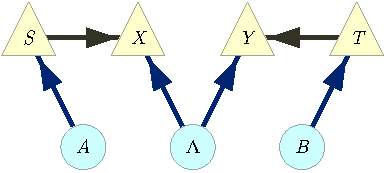
\includegraphics[width=2.55in]{GenuineBellDAG.pdf}
    \label{fig:BellDAG}
\end{minipage}}\hfill{\color{gray}\rule[-0.4cm]{0.5pt}{3cm}}\hfill
\subfigure[\hspace{-0.5ex}:\hspace{1ex} The \tred{latent reduction} of the Bell scenario. Influences between observables have been deleted, but every observable is now directly connected to all of its latent ancestors. See Fig.~1 in Ref. \cite{fritz2012bell}. \hfill]
{\begin{minipage}[t]{.45\textwidth}
    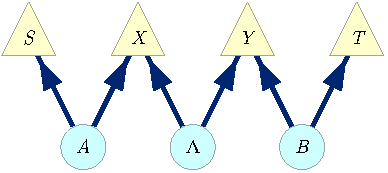
\includegraphics[width=2.55in]{EffectiveBellDAG.pdf}
    \label{fig:EffBellDAG}
\end{minipage}}
\vspace{-2ex}\caption{The Bell scenario: A scenario in which ${X}\cramp{\perp}{T}$ and ${Y}\cramp{\perp}{S}$ but ${X}\cramp{\not\perp}{Y}$. The Bell scenario is particularly famous in quantum theory \cite{bell1966lhvm,Brunner2013Bell,WoodSpekkens}, as many non-local correlations have be generated by replacing $\Lambda$ with some quantum $\bm\rho$.}
\label{fig:Bell}\vspace{-2ex}
\end{figure*}

Consider the causal structure associated to the Bell/CHSH \cite{bell1964einstein,Brunner2013Bell,bell1966lhvm,CHSHOriginal} experiment [\citealp{pusey2014gdag}~(Fig.~E\#2), \citealp{WoodSpekkens}~(Fig.~19), \citealp{chaves2014novel}~(Fig.~1), \citealp{BeyondBellII}~(Fig.~1), \citealp{wolfe2015nonconvexity}~(Fig.~2b), \citealp{steeg2011relaxation}~(Fig.~2)], depicted here in \cref{fig:BellDAG}. $\brackets{S,T,X,Y}$ are all observable variables and $\Lambda$ is the latent common cause of $X$ and $Y$.

%Without loss of generality let's assume that the values $\Lambda\mathopen{=}\lambda$ are drawn from some (possibly infinite, possibly continuous) set $\lambda\in\Omega$. 
The assumption of causal structure dictates that
\begin{align}\begin{split}\label{eq:bellstructure}
%\p{x y s t | \lambda a b}=\p{x_{\lambda a} y_{\lambda b} s_x t_y}
\p{x_{\lambda a b}}=\p{x_{\lambda a}} \,,\; \p{y_{\lambda a b}}=\p{y_{\lambda b}} \,,\; \p{s_{\lambda a b}}=\p{s_{a}} \,,\; \p{t_{\lambda a b}}=\p{t_{b}} \,,%\quad\text{and hence}\quad \p{x y s t | \lambda a b}=\p{x_{\lambda a} y_{\lambda b} s_x t_y}\,,
%=\p{x_{s|\lambda}}\p{y_{t|\lambda}}
\end{split}\end{align}
and hence
\begin{align}\begin{split}\label{eq:bellintegration}
&\p{x y s t | \lambda a b}=\p{x_{\lambda a} y_{\lambda b} s_a t_b}\,,\quad\text{and accordingly}\quad \p{x y s t}=\sum\limits_{{\lambda\in \norm{\Lambda}}}\sum\limits_{{a\in \norm{A}}}\sum\limits_{{b\in \norm{B}}}\p{x_{\lambda a} y_{\lambda b} s_a t_b}\p{\lambda}\p{a}\p{b}.
\end{split}\end{align}
These ancestral-latent dependencies per \cref{eq:bellstructure} are used to map the genuine Bell causal structure (\cref{fig:BellDAG}) to its latent reduction, namely \cref{fig:EffBellDAG}, which \tred{implies the same latent independencies}. The Bell causal structure is known to be lossless under latent reduction \citep[Thm.~2.4]{fritz2012bell}, so \cref{fig:BellDAG} and \cref{fig:EffBellDAG} are indeed observationally equivalent.

An important causal criterion is as follows. 
\begin{prop} \label{prop:CH}
The Bell causal structure (\cref{fig:Bell}) implies that
\begin{align*}
\p{x^1 y^1 s^1 t^1} \p{x^2 y^2 s^2 t^2}
\leq
\p{x^2 s^2 t^1} \p{x^1 y^3 s^1 t^2}
+\p{y^2 s^1 t^2} \p{x^3 y^1 s^2 t^1}
+\p{s^1 t^1} \p{\n{x^3} \n{y^3} s^2 t^2}
\end{align*}
\end{prop}

\begin{proof}
To prove \cref{prop:CH}, start with this logical tautology pursuant to \cref{fig:EffBellDAG}
\begin{align}\begin{split}
\NamedFunction{And}{ x^1_{\lambda ^1 a^1} , y^1_{\lambda ^1 b^1} , s^1_{a^1} , t^1_{b^1} , x^2_{\lambda ^2 a^2} , y^2_{\lambda ^2 b^2} , s^2_{a^2} , t^2_{b^2} }
\implies 
\NamedFunction{Or}{
    \NamedFunction{And}{ x^2_{\lambda ^2 a^2} , s^2_{a^2} , t^1_{b^1} , x^1_{\lambda ^1 a^1} , y^3_{\lambda ^1 b^2} , s^1_{a^1} , t^2_{b^2} } ,\\
    \NamedFunction{And}{ y^2_{\lambda ^2 b^2} , s^1_{a^1} , t^2_{b^2} , x^3_{\lambda ^1 a^2} , y^1_{\lambda ^1 b^1} , s^2_{a^2} , t^1_{b^1} } ,\\
    \NamedFunction{And}{ s^1_{a^1} , t^1_{b^1} , \n{x^3_{\lambda ^1 a^2}} , \n{y^3_{\lambda ^1 b^2}} , s^2_{a^2} , t^2_{b^2} } 
}
\end{split}\end{align}
which converts to the inequality
\begin{align}\begin{split}\label{eq:bellstructineq}
\p{x^1_{\lambda ^1 a^1} y^1_{\lambda ^1 b^1} s^1_{a^1} t^1_{b^1}} \p{x^2_{\lambda ^2 a^2} y^2_{\lambda ^2 b^2} s^2_{a^2} t^2_{b^2}}
\leq
\lparens{
\hphantom{+}\p{x^2_{\lambda ^2 a^2} s^2_{a^2} t^1_{b^1}} \p{x^1_{\lambda ^1 a^1} y^3_{\lambda ^1 b^2} s^1_{a^1} t^2_{b^2}}
\\+\p{y^2_{\lambda ^2 b^2} s^1_{a^1} t^2_{b^2}} \p{x^3_{\lambda ^1 a^2} y^1_{\lambda ^1 b^1} s^2_{a^2} t^1_{b^1}}
\\+\p{s^1_{a^1} t^1_{b^1}} \p{\n{x^3_{\lambda ^1 a^2}} \n{y^3_{\lambda ^1 b^2}} s^2_{a^2} t^2_{b^2}}
}
\end{split}\end{align}
or, equivalently,
\begin{align}
\p{x^1 y^1 s^1 t^1|\lambda ^1 a^1 b^1} \p{x^2 y^2 s^2 t^2|\lambda ^2 a^2 b^2}
\leq
\lparens{
\hphantom{+}\p{x^2 s^2 t^1|\lambda ^2 a^2 b^1} \p{x^1 y^3 s^1 t^2|\lambda ^1 a^1 b^2}
\\+\p{y^2 s^1 t^2|\lambda ^2 b^2 a^1} \p{x^3 y^1 s^2 t^1|\lambda ^1 a^2 b^1}
\\+\p{s^1 t^1|a^1 b^1} \p{\n{x^3} \n{y^3} s^2 t^2|\lambda ^1 a^2 b^2}
}\,.
\end{align}
To complete the proof we simply marginalize both sides over $\brackets{\lambda ^1, a^1, b^1,\lambda ^2, a^2, b^2}$.\end{proof}


A special case of \cref{prop:CH} is obtained by setting $\brackets{x^2,y^2}\to\mathsf{True}$, $x^3\to \n{x^1}$, and $y^3\to \n{y^1}$. This yields
\begin{align}
\p{x y s^1 t^1} \p{s^2 t^2}
\leq
\p{s^2 t^1} \p{x \n{y} s^1 t^2}
+\p{s^1 t^2} \p{\n{x} y s^2 t^1}
+\p{s^1 t^1} \p{x y s^2 t^2}
\end{align}
which is better understood in conditional form, namely
\begin{align}
\p{x y | s^1 t^1} \p{s^1 t^1}\p{s^2 t^2}
\leq
\p{x \n{y} | s^1 t^2}\p{s^1 t^2}\p{s^2 t^1} 
+\p{\n{x} y | s^2 t^1}\p{s^2 t^1}\p{s^1 t^2} 
+\p{x y | s^2 t^2}\p{s^2 t^2}\p{s^1 t^1}.
\end{align}
However, the Bell scenario causal structure further implies that $\p{s t}=\p{s}\p{t}$, and hence
\begin{align}
\p{x y | s^1 t^1}
\leq
\p{x \n{y} | s^1 t^2}
+\p{\n{x} y | s^2 t^1}
+\p{x y | s^2 t^2}.
\end{align}
Finally, we may eliminate negation notation entirely by substituting $\p{x \n{y} | s t} \to \p{x | s t}-\p{x y | s t} = \p{x | s}-\p{x y | s t}$ etc. Thus we obtain
\begin{align}
\p{x y | s^1 t^1} + \p{x y | s^1 t^2} + \p{x y | s^2 t^1}
\leq
\p{x | s^1}
+\p{y | t^1}
+\p{x y | s^2 t^2}.
\end{align}
which is simply the Clauser-Horne (CH) inequality \cite{CHInequality} for the Bell scenario. The CH inequality is the \emph{unique} Bell inequality (up to permutations) for the Bell scenario if $\brackets{S,T,X,Y}$ are all binary, and hence the CH inequality is a necessary and sufficient criterion to ascertain if correlations are compatible with that Bell scenario variant.











\section{Deriving inequalities algorithmically}

As evidenced, we derive polynomial inequalities in the observable variables by constructing logical tautologies (and their associated inequalities) in terms of conditional propositions. From the Bell scenario example it should be clear that the tautologies make use of the latent reduction. Therefore, the preliminary steps for deriving polynomial inequalities from $G$ are
\begin{compactenum}
\item Modify $G$ so that it is latent completed, if it isn't already.
\item Perform latent reduction to obtain $G'$.
\end{compactenum}

\bigskip
In algorithmically deriving polynomial inequalities we elect to sacrifice some generality in exchange for simplicity. In particular, we herein limit our consideration to tautologies of the ``supplemented excluded middle" (SEM) form. An excluded-middle (EM) tautology follows the following format: 
%\begin{align}
%Q1 \lor Q2 \lor Q3 \lor...\lor \parens*{\n{Q1}\land\n{Q2}\land\n{Q3}\land...}
%\end{align}
\begin{align}
\NamedFunction{Or}{Q1 , Q2 , Q3 ,..., \NamedFunction{And}{\n{Q1} ,\n{Q2},\n{Q3},...}}
\end{align}
An SEM tautology intersperses an EM tautology with a bunch of ``known" proposition, such as the following:
\begin{align}
%P1\land P2 \land P3 \land ... \implies \parens*{Q1\land P2\land P3} \lor \parens*{Q2\land P1\land P3} \lor \parens*{Q3\land P1\land P2} \lor...\lor \parens*{\n{Q1}\land\n{Q2}\land\n{Q3}\land ...}
\NamedFunction{And}{P1, P2 , P3 , ...} \implies 
\NamedFunction{Or}{
  \NamedFunction{And}{Q1, P2 , P3 , ...}
\\\NamedFunction{And}{P1, Q2 , P3 , ...}
\\\NamedFunction{And}{P1, P2 , Q3 , ...}
\\\NamedFunction{And}{\n{Q1} ,\n{Q2},\n{Q3},...}
}
\end{align}
The inequalities in terms of conditional events (such as \cref{eq:tri2structineq,eq:tri3structineq,eq:bellstructineq}) must satisfy the following requirements in order to correspond to SEM tautologies and still admit marginalization over the latent variables:
\begin{compactitem}[$\bullet$]
\item Every event on the right hand side of the inequality but not on the left hand side should appear negated in the final term on the left hand side. Such events are the ``unkowns" in the supplemented tautology of the excluded middle. 
%We've been highlighting them in the latent-complete inequalities presented here. 
We call the final term on the right hand side the ``closure" term, as it is closes the excluded middle tautology.

\item Every ``uknown" event (i.e. every event on the right hand side of the inequality but not on the left hand side) should appear in precisely \emph{one} non-closure term on the left hand side. No two such events are allowed in any single term, aside from the closure term, as this would (typically) break the tautology.\footnote{Any tautology of the form $\NamedFunction{And}{\_...}\cramp{\scriptstyle\implies}\NamedFunction{Or}{\NamedFunction{And}{\_...},\NamedFunction{And}{\_...},...}$ corresponds to a legitimate inequality. The SEM tautology is only the easiest to construct, but others are also possible.}

\item In every term, on both sides of the inequality, all instances of a latent variable with common dummy index must be restricted to the same joint probability. This is necessary in order to marginalize over the latent variables pursuant to the causal structure.
\end{compactitem}

While not strictly necessary, in order to make the inequality as compelling as possible one should ensure that every event on the left hand side should also be referenced on the right hand side. If one finds an inequality lacking this property, one can tighten it by using the special in which all such events are set to $\mathsf{True}$. Such choice substitution increases the probability of the left hand side without affecting the right hand side.

Note that these polynomial inequalities are not related whatsoever to the polynomial Bell inequalities recently introduced by \citet{ChavesPolynomial} and \citet{RossetNetworks}, nor to the interventional inequalities of \citet{kang2007polynomialconstraints} and \citet{steeg2011relaxation}.












\clearpage
\section{Other Causal Scenarios}
Here we present a few other causal structures of note and some polynomial inequalities which are justified by our method. Many more inequalities for these scenarios, and also additional scenarios, \purp{will be} considered in the Supplementary Materials.
\begin{figure*}
\centering
\subfigure[\hspace{-0.5ex}:\hspace{1ex} The causal structure of the S15 scenario. Implies ${Z}\cramp{\perp}{W}$. ${X}\cramp{\perp}{Y}|W$ is also implied if the dotted edges $A\to X$ and $A\to Y$ are absent. \hfill]
{\begin{minipage}[t]{.45\textwidth}
    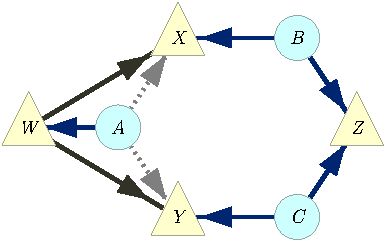
\includegraphics[width=2.55in]{GenuineS15DAG.pdf}
    \label{fig:S15DAG}
\end{minipage}}
\hfill{\color{gray}\rule[-0.4cm]{0.5pt}{3cm}}\hfill
%\hfill{\color{gray}\rule[-0.4cm]{0.5pt}{3cm}}$\quad\longmapsto\quad${\color{gray}\rule[-0.4cm]{0.5pt}{3cm}}\hfill
\subfigure[\hspace{-0.5ex}:\hspace{1ex} The latent reduction of the S15 scenario. Implies only ${Z}\cramp{\perp}{W}$. \hfill]
{\begin{minipage}[t]{.45\textwidth}
    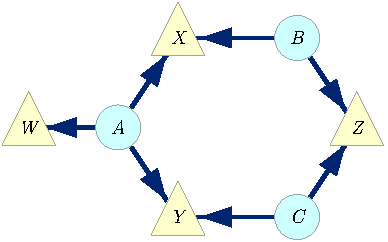
\includegraphics[width=2.55in]{EffectiveS15DAG.pdf}
    \label{fig:EffS15DAG}
\end{minipage}}
\vspace{-2ex}\caption{\purp{Two variants of the S15 scenario, so named because the ``empty" variant is listed as ``interesting" structure \#15 in Ref. \cite[Appx. E]{pusey2014gdag}. The ``empty" variant excludes the dotted edges, the ``full" variant includes them. The empty variant is lossy under latent reduction, but the full variant is lossless. Both variants have the same latent reduction.}\hfill
\\{\color{gray}\rule{\textwidth}{0.5pt}}
}
\label{fig:S15Scenario}\vspace{-3ex}
\end{figure*}




\begin{figure*}
\centering
\subfigure[\hspace{-0.5ex}:\hspace{1ex} The causal structure of the S20 scenario. Implies ${Z}\cramp{\perp}{W}$. ${Y}\cramp{\perp}{W}|X$ is also implied if the dotted edges $Z\to Y$ and $W\to Y$ are absent. \hfill]
{\begin{minipage}[t]{.45\textwidth}
    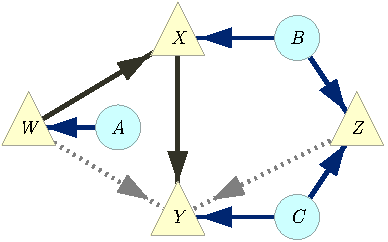
\includegraphics[width=2.55in]{GenuineS20DAG.pdf}
    \label{fig:S20DAG}
\end{minipage}}
\hfill{\color{gray}\rule[-0.4cm]{0.5pt}{3cm}}\hfill
%\hfill{\color{gray}\rule[-0.4cm]{0.5pt}{3cm}}$\quad\longmapsto\quad${\color{gray}\rule[-0.4cm]{0.5pt}{3cm}}\hfill
\subfigure[\hspace{-0.5ex}:\hspace{1ex} The latent reduction of the S20 scenario. Implies only ${Z}\cramp{\perp}{W}$.\hfill]
{\begin{minipage}[t]{.45\textwidth}
    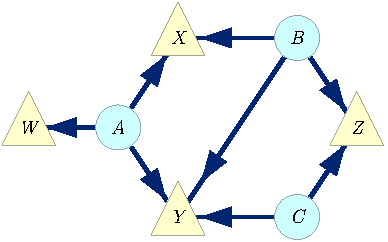
\includegraphics[width=2.55in]{EffectiveS20DAG.pdf}
    \label{fig:EffS20DAG}
\end{minipage}}
\vspace{-2ex}\caption{\purp{Two variants of the S20 scenario, so named because the ``empty" variant is listed as ``interesting" structure \#20 in Ref. \cite[Appx. E]{pusey2014gdag}. The ``empty" variant excludes the dotted edges, the ``full" variant includes them. The empty variant is lossy under latent reduction, but the full variant is lossless. Both variants have the same latent reduction.}\hfill
\\{\color{gray}\rule{\textwidth}{0.5pt}}
}
\label{fig:S20Scenario}\vspace{-3ex}
\end{figure*}


\begin{figure*}
\centering
\subfigure[\hspace{-0.5ex}:\hspace{1ex} The causal structure of the S7 scenario. Implies ${Z}\cramp{\perp}{W}$.\hfill]
{\begin{minipage}[t]{.45\textwidth}
    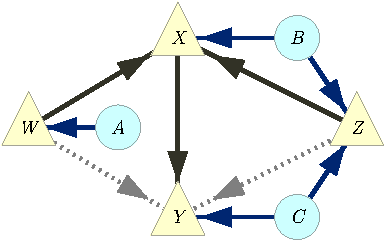
\includegraphics[width=2.55in]{GenuineS7DAG.pdf}
    \label{fig:S7DAG}
\end{minipage}}
\hfill{\color{gray}\rule[-0.4cm]{0.5pt}{3cm}}\hfill
%\hfill{\color{gray}\rule[-0.4cm]{0.5pt}{3cm}}$\quad\longmapsto\quad${\color{gray}\rule[-0.4cm]{0.5pt}{3cm}}\hfill
\subfigure[\hspace{-0.5ex}:\hspace{1ex} The latent reduction of the S7 scenario. Implies ${Z}\cramp{\perp}{W}$.\hfill]
{\begin{minipage}[t]{.45\textwidth}
    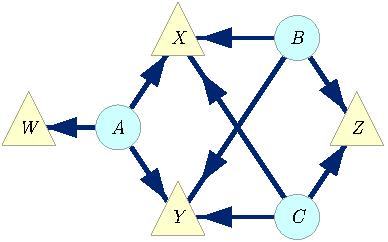
\includegraphics[width=2.55in]{EffectiveS7DAG.pdf}
    \label{fig:EffS7DAG}
\end{minipage}}
\vspace{-2ex}\caption{\purp{Two variants of the S7 scenario, so named because the ``empty" variant is listed as ``interesting" structure \#7 in Ref. \cite[Appx. E]{pusey2014gdag}. The ``empty" variant excludes the dotted edges, the ``full" variant includes them. Both variants are lossy under latent reduction; both variants have the same latent reduction.}\hfill
}
\label{fig:S7Scenario}\vspace{-2ex}
\end{figure*}


\begin{prop}\label{prop:S15deg2example}
The S7 causal structure (\cref{fig:S7Scenario}) implies that
\begin{align*}
&\p{w^1} \p{w^2} \p{x y z^1 w^3}
\leq
{
\p{w^2} \p{z^2 w^1} \p{x y z^1 w^3}
+\p{w^1} \p{\n{z^2} w^2} \p{x y z^1 w^3}
}\,.
%\end{align*}
%\begin{align*}
\\\hspace{-\mathindent}\textit{Proof.}\qquad &\p{w^1_{a^1}} \p{w^2_{a^3}} \p{x_{a^2 b^2 c^2} y_{a^2 b^2 c^2} z^1_{b^2 c^2} w^3_{a^2}}
\leq
\lparens{
\hphantom{+}\p{w^2_{a^3}} \p{z^2_{b^1 c^3} w^1_{a^1}} \p{x_{a^2 b^2 c^2} y_{a^2 b^2 c^2} z^1_{b^2 c^2} w^3_{a^2}}
\\+\p{w^1_{a^1}} \p{\n{z^2_{b^1 c^3}} w^2_{a^3}} \p{x_{a^2 b^2 c^2} y_{a^2 b^2 c^2} z^1_{b^2 c^2} w^3_{a^2}}
}\,.
\end{align*}
\end{prop}

\clearpage
\begin{acknowledgments}
%\bigskip\noindent\textbf{Acknowledgments}
Research at Perimeter Institute is supported by the Government of Canada through Industry Canada and by the Province of Ontario through the Ministry of Economic Development and Innovation.
\end{acknowledgments}

%\section*{References}
%\nocite{*}
%\setlength{\bibsep}{\smallskipamount}
\setlength{\bibsep}{3pt plus 3pt minus 2pt}
\bibliographystyle{apsrev4-1}
\nocite{apsrev41Control}
\bibliography{apsrevcontrol,hardyinference}


\onecolumngrid
\appendix
\renewcommand{\theequation}{A-\arabic{equation}}
\setcounter{equation}{0}


%%%%%%%%%%%% Enumeration via lowercase letters
\renewcommand{\labelenumi}{(\alph{enumi})}
\renewcommand{\theenumi}{(\alph{enumi})}
\renewcommand{\labelitemi}{$\circ$}

\section{Tobias's Original 7 Inequalities}

``I present several inequalities... together with a method of proof which has a combinatorial flavour. No quantum violations of any of these inequalities has been found to date.

In the following the complement of a value is marked by an empty circle accent, so $\mathring{b}$ means ``anything but $b$", and accordingly $P(\mathring{a}\mathring{b})=P(A\mathopen{\neq}a,B\mathopen{\neq}b)$. 
%Additionally, an underscore stands for the corresponding marginal probability, like this: $P(\_b\_) := P(abc) + P(ab\mathring{c}) + P(\mathring{a}bc) + P(\mathring{a}b\mathring{c})$. 
\begin{theorem}
The following inequalities hold for all classical correlations in the triangle scenario:
\begin{enumerate}
\item
\(\quad
%--(a)--
%P(0\_\_)P(\_\_1) \leq P(00\_)+P(\_11)
P(a) P(c)  \leq  P(a b) + P(\nb c)
\)
\item
\(\quad
%--(b)--
%P(001) P(010) P(100)  \leq  P(000) + P(11\_) P(001) P(0\_\_) + P(1\_1) P(010) P(\_\_0) + P(\_11) P(100) P(\_0\_)
P(a b\nc) P(a \nb c) P(\na b c) \leq P(a b c) + P(\na \nb) P(a b \nc) P(a) + P(\na\nc) P(a\nb c) P(c)  + P(\nb \nc) P(\na b c) P(b)
\)
\item 
\(\quad
%--(c)--
%P(001) P(010) P(100) \leq  P(000)^2 + 2 P(11\_) P(001) + 2 P(1\_1) P(010) + 2 P(\_11) P(100)
P(a b\nc) P(a \nb c) P(\na b c) \leq P(a b c)^2 + 2\parens*{P(\na \nb) P(a b \nc) + P(\na\nc) P(a\nb c)  + P(\nb \nc) P(\na b c)}
\)
\item
\(\quad
%--(d)--
%P(000)^2 P(111)  \leq  P(001) P(010) P(100) + (2 P(000) + P(111)) (1 - P(000) - P(111))
P(a b c)^2 P(\na\nb\nc)  \leq  P(a b \nc) P(a \nb c) P(\na b c) + \parens*{2 P(a b c) + P(\na\nb\nc)} \parens*{1 - P(a b c) - P(\na\nb\nc)}
\)
\item
\(\quad
%--(e)--
%P(000)^2 P(111)  \leq  P(000)^3 + (2 P(000) + P(111)) (1 - P(000) - P(111))
P(a b c)^2 P(\na\nb\nc)  \leq  P(a b c)^3 + \parens*{2 P(a b c) + P(\na\nb\nc)} \parens*{1 - P(a b c) - P(\na\nb\nc)}
\)
\item
\(\quad
%--(f)--
%P(1\_\_)P(\_1\_)P(\_\_1) \leq P(000)+P(11\_)P(\_\_1)+P(1\_1)P(\_1\_)+P(\_11)P(1\_\_)
P(a) P(b) P(c) \leq  P(\na\nb\nc) + P(a b) P(c) + P(a c) P(b) + P(b c) P(a)
\)
\item
\(\quad
%--(g)--
%P(1\_\_)P(\_1\_)P(\_\_1) \leq P(000)^2+2 P(11\_)P(\_\_1) + 2 P(1\_1)P(\_1\_) + 2 P(\_11)P(1\_\_)
P(a) P(b) P(c) \leq  P(\na\nb\nc)^2 +2\parens[\Big]{ P(a b) P(c) + P(a c) P(b) + P(b c) P(a) }
\)
\end{enumerate}
\end{theorem}

It is quite likely that some of these inequalities are dominated by the others, but I do not know for sure whether any of them are actually redundant."

\purp{Note that \cref{prop:AllPowerful} implies inequalities (a), (b), and (f). I haven't checked the others yet. \quoteby EW}

\begin{comment}
\section{Copy and Paste Playground}
\begin{align}
\parens{
    {x}_{s^0}^{\lambda ^2} , {x}_{s^0}^{\lambda ^1} , {y}_{t^0}^{\lambda ^1}
}
&\implies 
\NamedFunction{Or}{
    \n{{y}_{t^1}^{\lambda ^2}} ,\\
     \parens{
        {x}_{s^0}^{\lambda ^1} , {y}_{t^0}^{\lambda ^1} , {x}_{s^0}^{\lambda ^2} , {y}_{t^1}^{\lambda ^2}
    }
} \\
\parens{
    {x}_{s^0}^{\lambda ^1} , {y}_{t^0}^{\lambda ^1} , {x}_{s^0}^{\lambda ^2} , {y}_{t^0}^{\lambda ^2}
}
&\implies 
\NamedFunction{Or}{
    \parens{
        \n{{x}_{s^1}^{\lambda ^2}} , \n{{y}_{t^1}^{\lambda ^1}}
    } ,\\
     \parens{
        {x}_{s^0}^{\lambda ^2} , {x}_{s^0}^{\lambda ^1} , {y}_{t^1}^{\lambda ^1}
    } ,\\
     \parens{
        {x}_{s^0}^{\lambda ^1} , {y}_{t^0}^{\lambda ^1} , {x}_{s^1}^{\lambda ^2} , {y}_{t^0}^{\lambda ^2}
    }
}\\
\parens{
    {x}_{s^0}^{\lambda ^1} , {y}_{t^0}^{\lambda ^1} , {x}_{s^0}^{\lambda ^2} , {y}_{t^0}^{\lambda ^2}
}
&\implies 
\NamedFunction{Or}{
    \parens{
        \n{{x}_{s^1}^{\lambda ^2}} , \n{{y}_{t^1}^{\lambda ^2}}
    } ,\\
     \parens{
        {x}_{s^0}^{\lambda ^1} , {y}_{t^0}^{\lambda ^1} , {x}_{s^0}^{\lambda ^2} , {y}_{t^1}^{\lambda ^2}
    } ,\\
     \parens{
        {x}_{s^0}^{\lambda ^1} , {y}_{t^0}^{\lambda ^1} , {x}_{s^1}^{\lambda ^2} , {y}_{t^0}^{\lambda ^2}
    }
}
\end{align}
\end{comment}
\end{document}